\documentclass[12pt]{article}

% Sprache, Encoding & Fonts
\usepackage[utf8]{inputenc}
\usepackage[T1]{fontenc}

% Layout & Grundpakete
\usepackage{geometry}
\geometry{margin=1in}
\usepackage{fullpage} % optional; geometry setzt Margin
\usepackage{setspace}
\usepackage{parskip}

% Mathematik & Symbole
\usepackage{amsmath,amssymb,amsthm}
\usepackage{mathrsfs}

% Grafiken & Plots
\usepackage{graphicx}
\graphicspath{{./resources/images/}}
\usepackage{caption}
\usepackage{subcaption}
\usepackage{float}
\usepackage{pgfplots}
\pgfplotsset{compat=newest}
\usepackage{tikz}
\usetikzlibrary{calc,intersections,decorations.pathreplacing,patterns,angles,quotes,shapes,arrows,positioning,automata}
\usepgfplotslibrary{fillbetween}

% Sonstige
\usepackage{enumitem}
\usepackage{booktabs}
\usepackage{multicol}
\usepackage{multirow}
\usepackage{polynom}
\usepackage{tikz-cd}
\usepackage{comment}
\usepackage{fancyvrb}
\usepackage{fancyhdr}
\usepackage{etoolbox}
\usepackage{listings}
\usepackage{tkz-euclide}
\usepackage{float}
\usepackage{hyperref}
\usepackage{siunitx} % für circuitikz/si-Einheiten falls benötigt
\usepackage{circuitikz} % optional, behält Option ohne Fehler

% Header/Footer
\pagestyle{fancy}
\fancyhead[l]{Gruppe 12}
\fancyhead[c]{SWT \#3}
\fancyhead[r]{\today}
\fancyfoot[c]{\thepage}
\renewcommand{\headrulewidth}{0.2pt}
\setlength{\headheight}{15pt}

% pgfplots etc.
\pgfplotsset{compat=1.18}

\begin{document}

\textbf{Rollen}

\begin{itemize}
  \item Fahrten-Anbietende: bieten eine Fahrt an
  \item Fahrten-Suchende: suchen und buchen
  \item Mitfahrende: haben eine Buchung
\end{itemize}

\textbf{Kern-Use-Cases (funktional)}

\textbf{Fahrt anlegen (Anbietende)}

Felder: Start/Ziel (Campus/Adresse), Datum \& Uhrzeit, freie Plätze, kurzer Hinweis (z.\,B. „Treffpunkt Mensa“, „kein Rauchen“), optional Kostenbeitrag (reiner Kostenausgleich).

\begin{itemize}
  \item \textit{include} Start/Ziel wählen, Plätze festlegen
  \item \textit{extend} Fahrt löschen/ändern (bis X Std. vorher)
\end{itemize}

\textbf{Fahrt suchen \& filtern (Suchende)}\\
Filter: Campus (Aachen/Jülich), Datum/Uhrzeit-Fenster, max. Umweg (z.\,B. +10 Min.), Plätze $\geq 1$.

\begin{itemize}
  \item \textit{include} Ergebnisliste anzeigen, Details ansehen
  \item \textit{extend} Such-Abo anlegen (Push bei neuen Treffern)
\end{itemize}

\textbf{Fahrt anfragen / Platz reservieren (Suchende → Anbietende)}\\
Ein-Klick-Anfrage mit kurzem Text (optional).

\begin{itemize}
  \item \textit{include} Benachrichtigung senden
  \item \textit{extend} Anfrage zurückziehen
\end{itemize}

\textbf{Anfragen annehmen/ablehnen (Anbietende)}\\
Plätze zählen sich automatisch herunter.

\begin{itemize}
  \item \textit{include} Bestätigung an Mitfahrende senden
\end{itemize}

\textbf{Kontakt aufnehmen (alle mit Bezug zur Fahrt)}\\
Minimaler Chat-Thread zur Abstimmung von Treffpunkt/Verspätung.

\begin{itemize}
  \item \textit{include} Push-Benachrichtigung
\end{itemize}

\textbf{Buchung verwalten (Mitfahrende)}\\
Buchung anzeigen, stornieren (bis Frist X).

\begin{itemize}
  \item \textit{extend} No-Show melden (nur für spätere Qualitätssicherung)
\end{itemize}

\textbf{Nicht-funktionale Mindestanforderungen}

\begin{itemize}
  \item \textbf{Login/Verifizierung:} E-Mail-Login, optional FH-Mail-Verifizierung (Trust-Bonus)
  \item \textbf{Datenschutz \& Rechtliches:} DSGVO-konforme Profile, klare AGB (Privat-Mitnahme, kein gewerblicher Transport)
  \item \textbf{Usability:} Mobile-first UI, Push-Notifications, klare Treffpunkt-Infos
  \item \textbf{Sicherheit/Moderation (light):} Melden-Button für Fahrt/Profil, einfache Sperrlogik
  \item \textbf{Stabilität:} Basis-Monitoring, Rate-Limiting für Spam-Schutz
\end{itemize}

\textbf{Tipp zur Diagramm-Anbindung}

\begin{itemize}
  \item Fahrt buchen \textit{include} Kontakt aufnehmen
  \item Fahrt suchen \textit{extend} Such-Abo anlegen
  \item Fahrt anlegen \textit{extend} Fahrt ändern/löschen
\end{itemize}

\textbf{Ausbaustufe 1 – Vertrauen \& Wiederkehr erhöhen}

\begin{itemize}
  \item \textbf{Bewertungen \& Profile:} Sterne + kurzer Kommentar nach der Fahrt; einfache Profilabzeichen (FH-Mail verifiziert, „100+ km unfallfrei“ o.\,ä.)
  \item \textbf{Serienfahrten:} Wöchentliche Pendelfahrten (z.\,B. Mo–Fr 08:00 → Campus), Auto-Wiederveröffentlichung
  \item \textbf{Live-Ankunftsstatus:} „Unterwegs“, ETA-Teilen (ohne permanentes Tracking)
  \item \textbf{Kalender-Integration:} Export/Import (iCal); Campus-Events als Zielvorschläge
  \item \textbf{Sicherheitsfeatures:} Notfall-Kontakt teilen, anonymer Chat-Alias (Telefonnummer bleibt verborgen)
\end{itemize}

\textbf{Ausbaustufe 2 – Skalierung \& Monetarisierung}

\begin{itemize}
  \item \textbf{In-App-Zahlungen (Kostenteilung):} SEPA/PayPal, automatische Split-Zahlung, Quittungen
  \item \textbf{Smart-Matching:} Zwischenstopps vorschlagen, Multi-Hop (Umstieg), Routen-Snapping, Priorisierung nach Umweg-Kosten
  \item \textbf{CO\textsubscript{2}-Tracking \& Anreize:} Einsparungen anzeigen; Teilnahme an FH/AStA-Programmen (Badges, kleine Benefits)
  \item \textbf{ÖPNV-/Park-Integration:} AVV-Verknüpfung (letzte Meile), Campus-Parkplätze/Belegung als Info
  \item \textbf{Organisationen \& Gruppen:} Fakultäts-/Kurs-Gruppen, Zugang per Einladungslink, Fahrten nur für Gruppe sichtbar
\end{itemize}

\textbf{Kurzbegründung (warum so?)}

\begin{itemize}
  \item \textbf{MVP:} deckt die minimale End-to-End-Kette ab: Fahrt anbieten → finden → anfragen → bestätigen → treffen
  \item \textbf{Stufe 1:} baut Vertrauen und Retention auf (Bewertungen, Serienfahrten, ETA)
  \item \textbf{Stufe 2:} schafft Komfort, Skalierung und ggf. Einnahmequellen (Payments, Matching, Integrationen)
\end{itemize}

% Beispielabbildungen: mit Breitenbegrenzung, damit nichts überläuft
\begin{figure}[H]
  \centering
  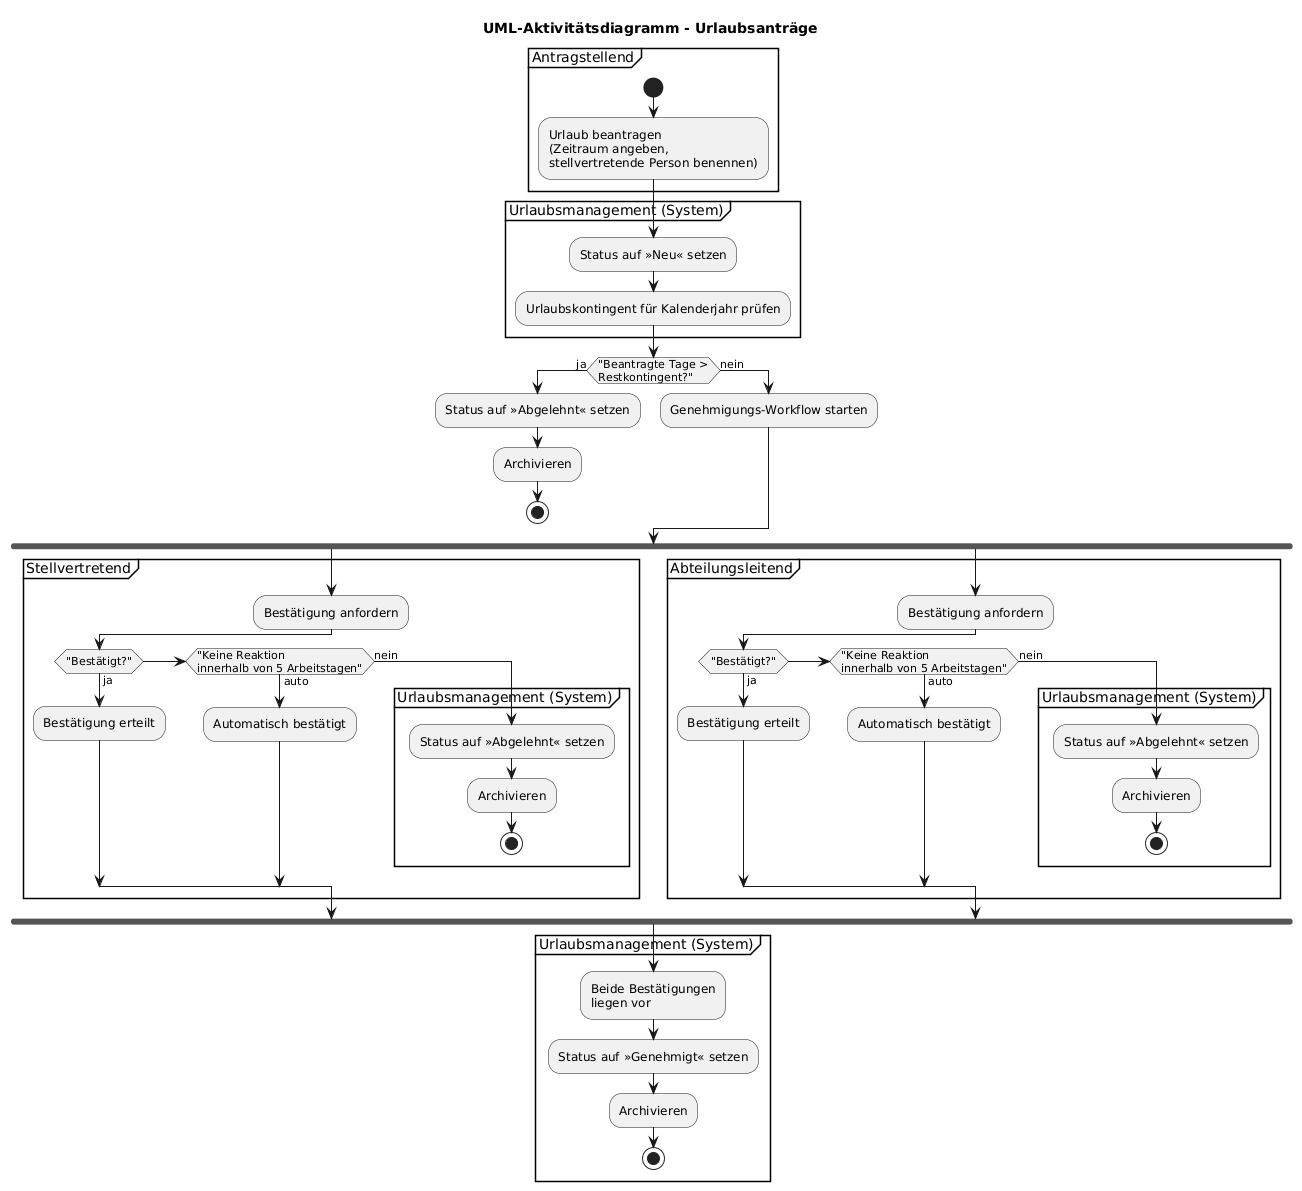
\includegraphics[width=\linewidth,keepaspectratio]{2.png}
  \caption{Abbildung 2}
\end{figure}

\begin{figure}[H]
  \centering
  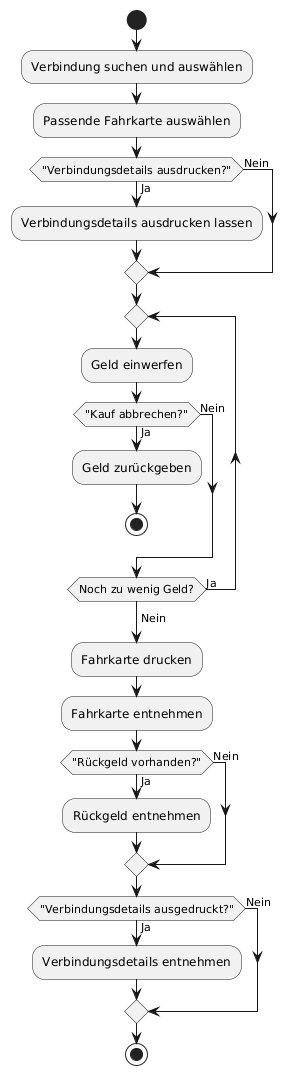
\includegraphics[width=\linewidth, height=0.9\textheight,keepaspectratio]{3.png}
  \caption{Abbildung 3}
\end{figure}

\begin{figure}[H]
  \centering
  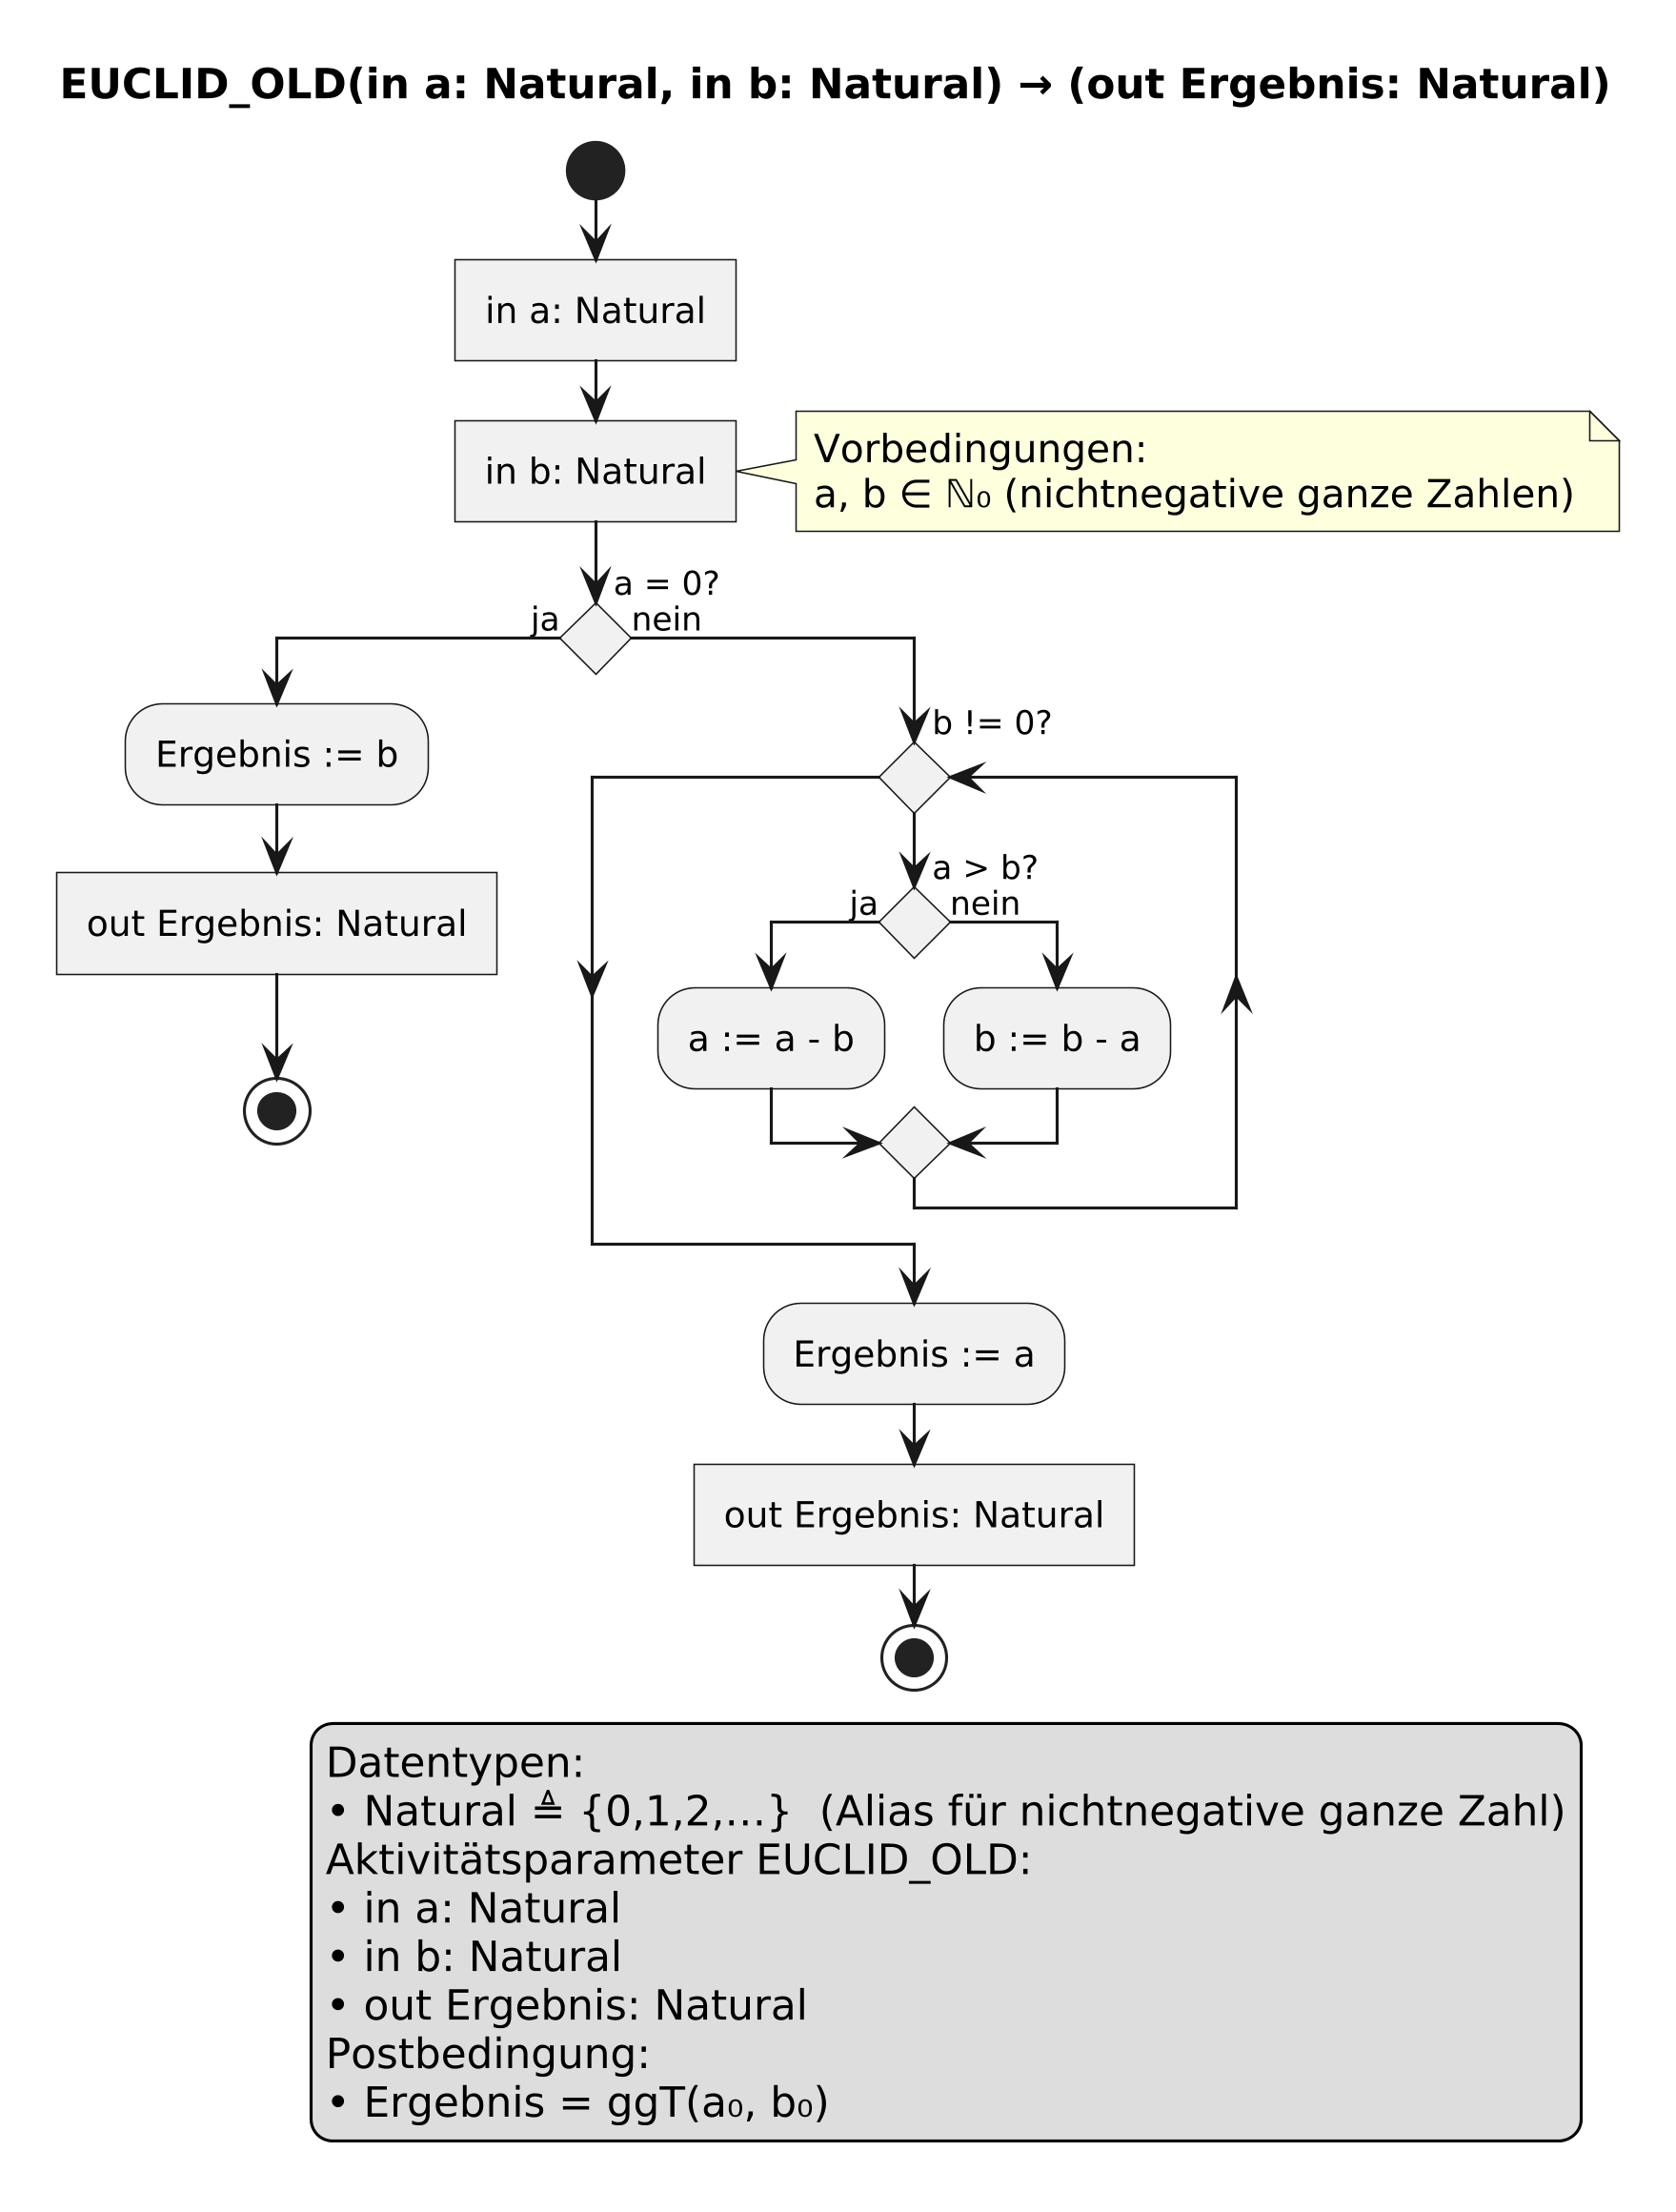
\includegraphics[width=\linewidth,keepaspectratio]{4.png}
  \caption{Abbildung 4}
\end{figure}

\end{document}
